\subsection{Expected and observed event yields}
\par After the event selection criteria for the signal region was finalized, and the background 
modelling validated, final kinematic distributions in the signal region were examined. 
Figure~\ref{fig:exclHsr} shows n-1 distributions for \dFem, \memu, \mT\ and \pTemu. 
N-1 distributions show event yields and shapes in the signal region, minus the 
selection criteria specific to the distribution being plotted. All the scale factors 
discussed in the preceding sections were applied to correctly model the backgrounds. 
For the exclusive \WW\ process, \fgam\ was multiplied by 1.57 to match validation 
results observed in Section~\ref{sec:exclHCR}. The inclusive \WW\ process was scaled 
by 0.79. As discussed in Section~\ref{sec:incWW}, applying this background implicitly 
adds the \Ztau\ background to the inclusive \WW\ background. The rest of the backgrounds 
were scaled by their respective scale factors to account for the mis-modelling of the 
underlying event in simulation.

\par A summary of the yields in the signal region is shown in Table~\ref{tab:Higgsyields}.    
Six events were observed in data, while 3.00$\pm$0.78 events were expected from all 
the background processes; 0.023$\pm$0.003 events were expected from signal, where the 
quoted uncertainty is the sum in quadrature of systematic uncertainties and simulation 
statistical uncertainties. 

\begin{table}[!h]
\centering
        \resizebox{\textwidth}{!}{
\providecommand{\cutflowTitle}{}
\begin{tabular}{|l|rrr|rrr|}
\hline
 																							& Excl. $H$ Signal				& Data 		& Total Bkg 		& Incl. $\WW$ 	& Excl. $W^{+}W^{-}$ & Other Bkg 								 \\
\hline\hline
Preselection 																	& 0.065 $\pm$ 0.005 			& 129018 	& 120090				& 12844 				& 43  								& 107200\\
 $\pTemu>$30~\GeV, $\memu<55$~\GeV, $\dFem<1.8$ & 0.043 $\pm$ 0.004 			& 18568 	& 17060  				& 2026 					& 5.7									& 15030 \\
\DZ\ requirement 															& 0.023 $\pm$ 0.003 			& 8 			& 4.7 $\pm$ 1.3 & 1.4 $\pm$ 0.5 & 3.1 $\pm$ 1.3       & 0.2 $\pm$ 0.1  \\
$\mT<140$~\GeV [Signal Region] 							& 0.023 $\pm$ 0.003  			& 6 			& 3.0 $\pm$ 0.8 & 1.0 $\pm$ 0.4 & 1.8 $\pm$ 0.8       & 0.2 $\pm$ 0.1  \\
\hline
\end{tabular}
}
\caption{Summary of signal and background yields at different stages
  of the Higgs boson event selection. Only major background sources are listed explicitly. All 
the other background sources are summed up in the `Other'
category. For the background, the uncertainties are only shown for the yields after exclusivity selection, where they are 
relevant for the measurement. They include the systematic and
statistical components, added in quadrature.}
\label{tab:Higgsyields}
\end{table}

\begin{figure}[!h]
\begin{subfigure}{0.5\textwidth}
   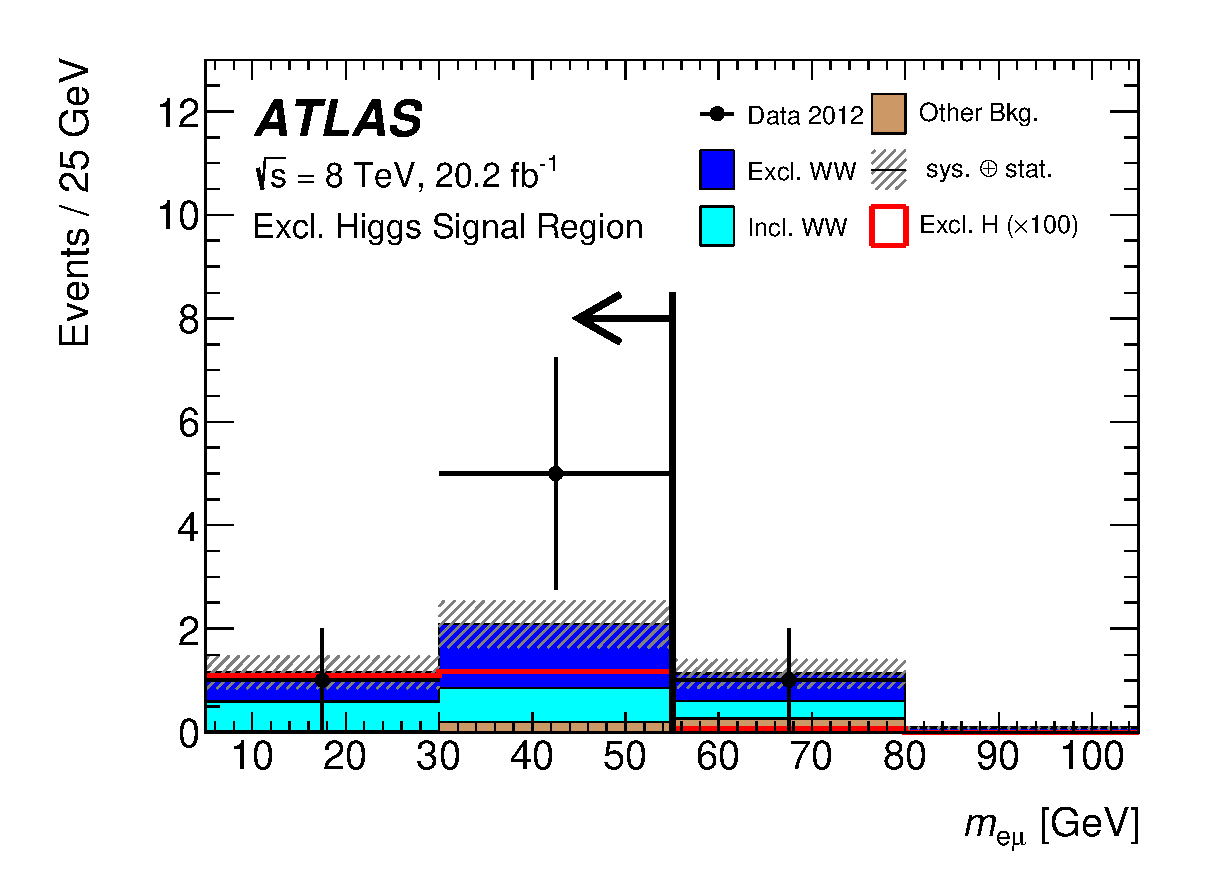
\includegraphics[width=\textwidth]{figures/emme_CutSR_Mll_nMinus1_MllnMinusOne.eps}
\end{subfigure}
\begin{subfigure}{0.5\textwidth}
   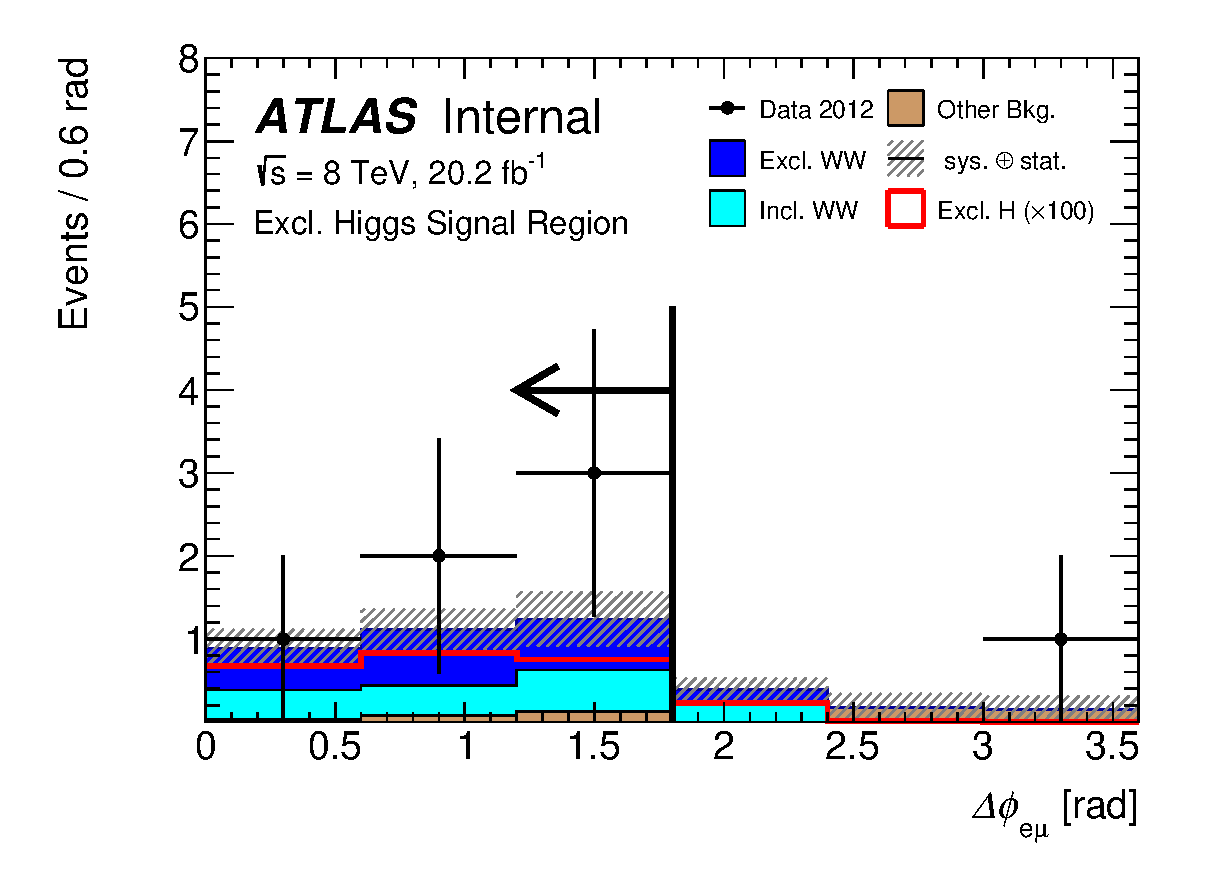
\includegraphics[width=\textwidth]{figures/emme_CutSR_DPhill_nMinus1_DPhillnMinusOne.eps}
\end{subfigure} 
\begin{subfigure}{0.5\textwidth}
   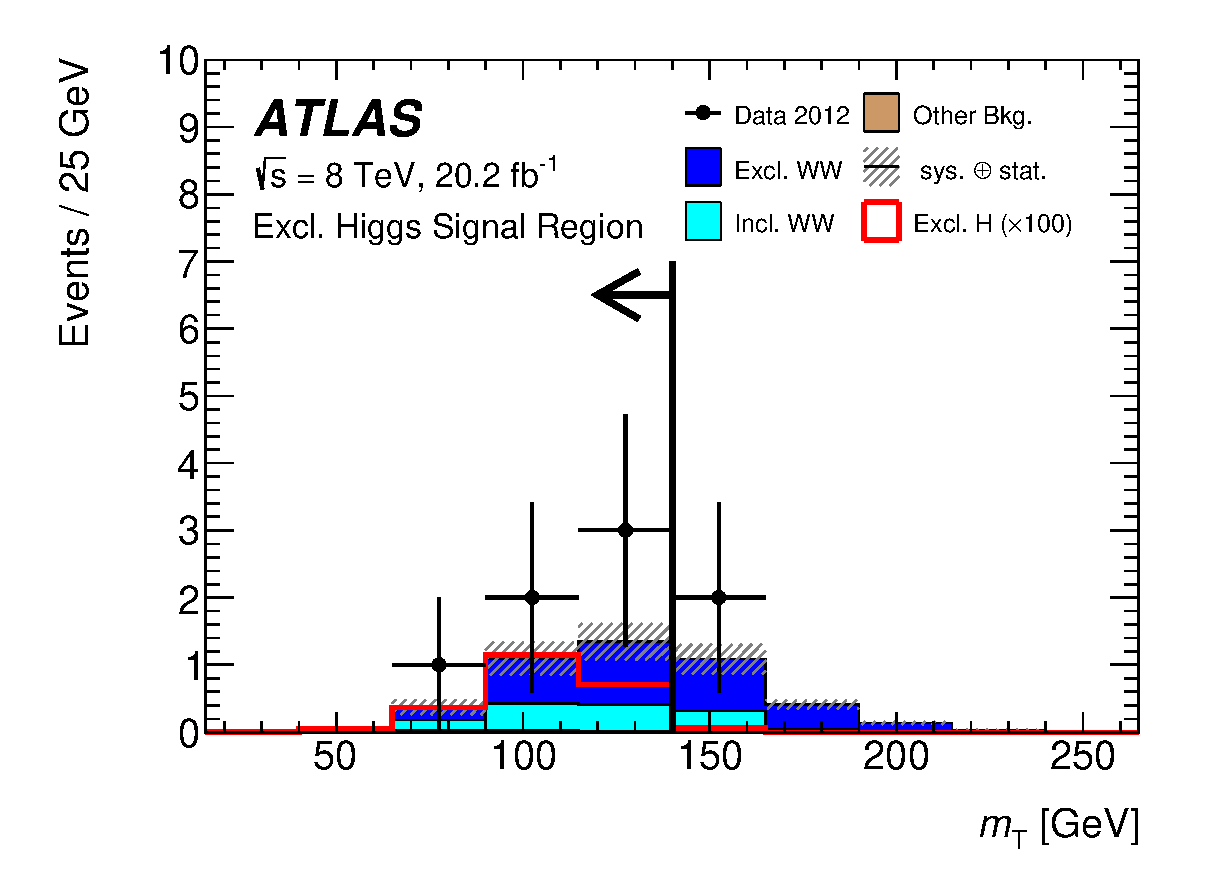
\includegraphics[width=\textwidth]{figures/emme_CutSR_MT_nMinus1_MTexcl.eps}
\end{subfigure} 
\begin{subfigure}{0.5\textwidth}
   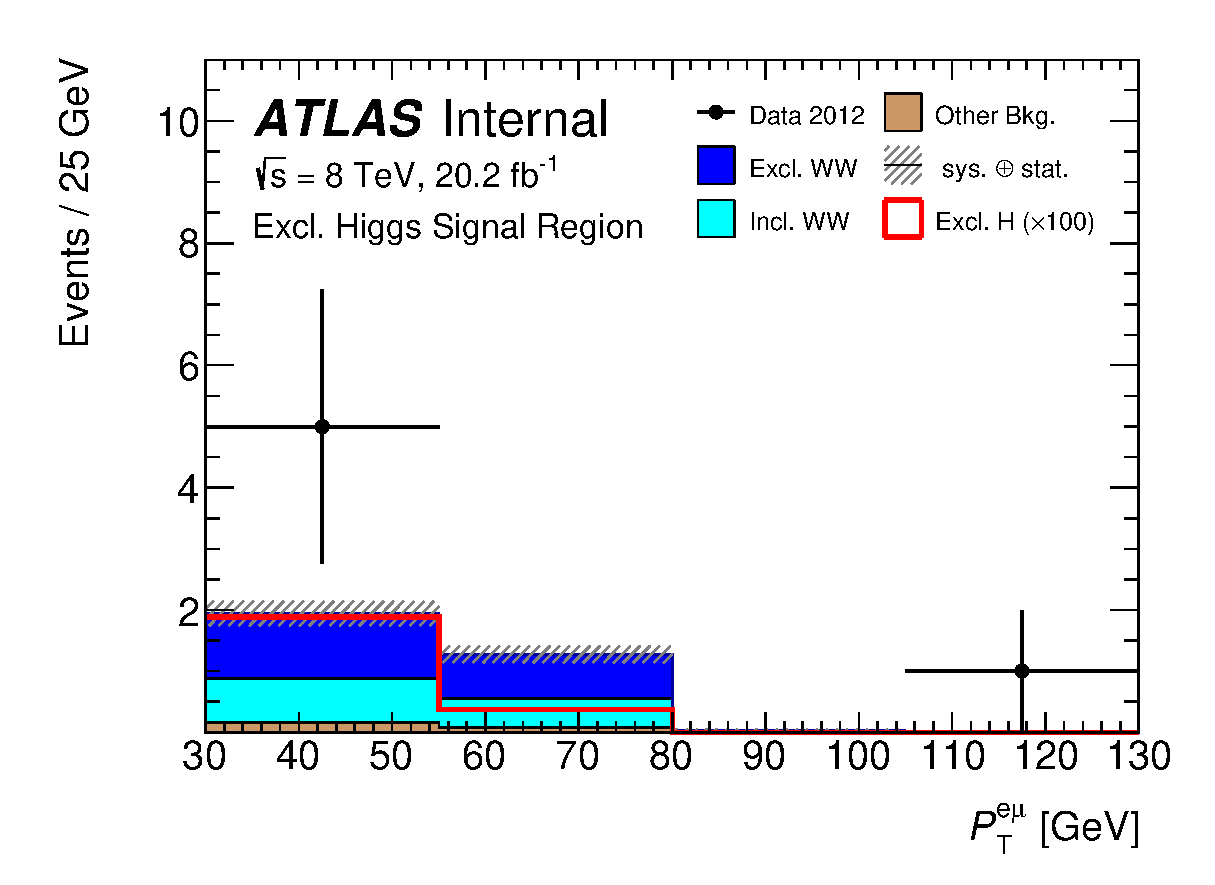
\includegraphics[width=\textwidth]{figures/emme_CutSR_Ptll_nMinus1_PtllnMinusOne_130.eps}
\end{subfigure} 
\caption{Plots showing \memu, \dFem, \mT\ and \pTemu\ distributions in the signal region, minus the selection criteria for the variable 
being plotted}
\label{fig:exclHsr}
\end{figure}


\subsection{Statistical Analysis}
\par The results presented in the preceding sub-section were tested for evidence of exclusive Higgs 
production in LHC Run I data. For a Standard Model Higgs boson with $m_{\text{H}} = 125~\GeV$, 
$\sigma^{Exp}_{H}$ was set at 
1 to make the parameter of interest $\mu=\sigma^{Obs}_{H}$. The test statistic $q_0$, where $\mu=0$ 
in Equation~\ref{eq:testStat}, was used to test the compatibility 
of observed data with the background-only hypothesis. The rest of the statistical analysis is identical 
to that described in Section~\ref{sec:chStat}, including the treatment of systematic uncertainties.
The discrepancy between the observed data and expected event yields corresponded to a 1.1$\sigma$ 
upward fluctuation from the expected Standard Model results. This fluctuation is not significant enough 
to prove existence of the exclusive Higgs boson. Expected limits on the exclusive Higgs boson 
cross section were therefore set, using the $CL_s$ procedure, where $CL_s(\mu)$ is defined as in Equation~\ref{eq:cls}. 

\par Table~\ref{tab:models} shows a summary of the 95\% CL upper limits on the exclusive 
Higgs boson total production cross-section.
The observed upper limit is 1.2 pb, which is 1.1$\sigma$ higher than the expected 
upper limit of 0.7 pb. The statistical uncertainty in the predicted background dominates the
uncertainty involved in calculating this upper limit, 
while systematic uncertainties worsen the upper limits by at most 10\%.
This upper limit value is 400 times the cross-section predicted~\cite{Khoze}.
However, the limit would not change if the model prediction, which is for
elastic production only, increased by an order of magnitude. This limit calculation 
inherently assumes that the acceptance and efficiency for dissociative
events is not significantly different than for elastic events, hence
the associated systematic uncertainty is insignificant.

\begin{table}
\centering
%\resizebox{0.5\textwidth}{!}{
\begin{tabular}{|cc|c|cc||r|}
\hline
$+2\sigma$ [pb] & $+1\sigma$ [pb] & Expected [pb] & $-1\sigma$ [pb] & $-2\sigma$ [pb] & Observed [pb] \\
\hline\hline
 1.6 & 1.0  & 0.7 &  0.5 &  0.4 & 1.2 \\
\hline 
\end{tabular}
%}
\caption{Upper limits on $\sigma_H$ [pb] at 95\% CL. The $\pm 1\sigma$ and $\pm 2\sigma$ uncertainties quoted here are on the expected upper limit.}
\label{tab:models}
\end{table}
